\begin{figure}[!ht]
	\centering
	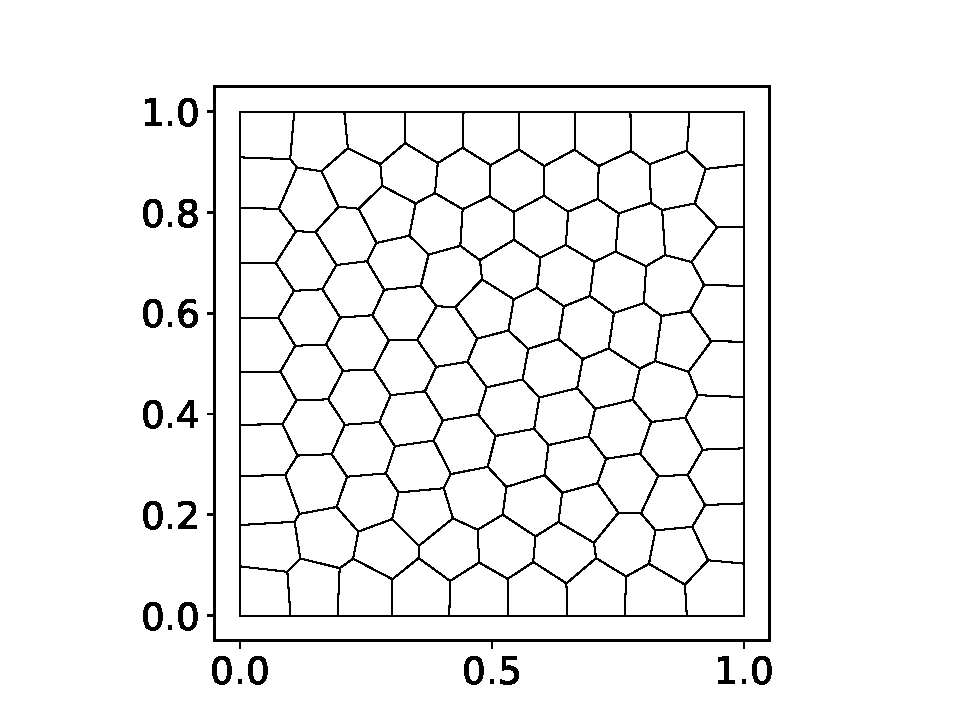
\includegraphics[trim=0cm 0.5cm 0cm 0.5cm, clip, width=7.5cm]{square_100.pdf}
    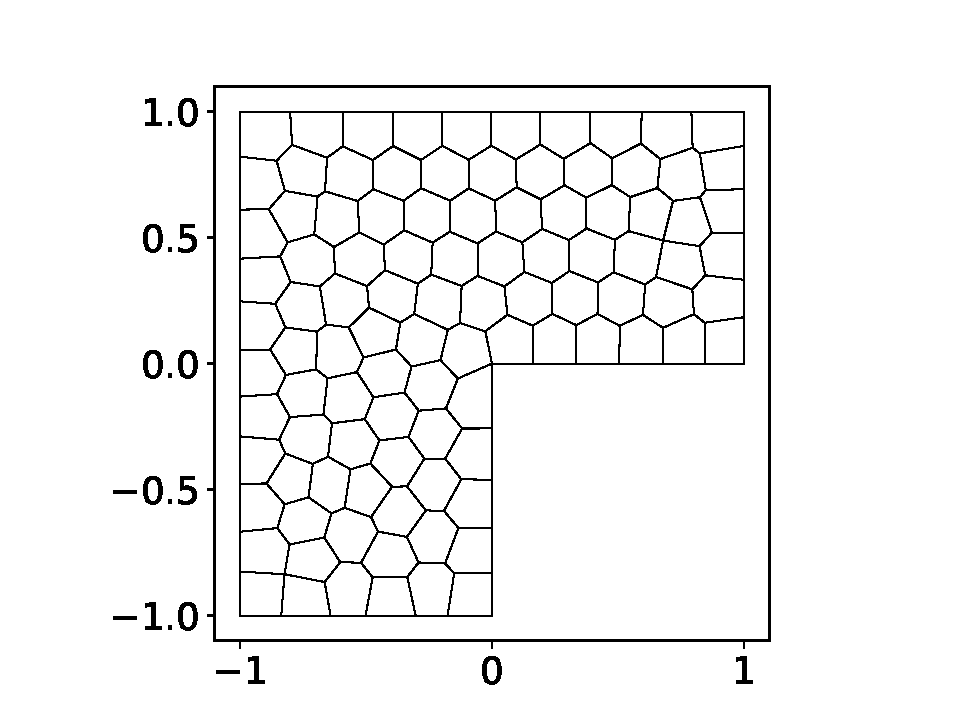
\includegraphics[trim=0cm 0.5cm 0cm 0.5cm, clip, width=7.5cm]{lshape_100.pdf}
	\caption{Square and L-shaped meshes over polygonal domains with 100 elements.}
\end{figure}

Meshes are fundamental tools in Finite Element algorithms. This algorithm utilizes polygonal meshes over a polygonal domain.

\cite{Talischi2012} Meshes are typically constructed by evaluating the Voronoi diagram of a random set of points within a polygon. This diagram is then relaxed using Lloyd's algorithm, which involves re-evaluating the Voronoi diagram of the centroids of the Voronoi cells and iterating until convergence is achieved based on a specified tolerance.

Meshes require a diagram, which is created or loaded using \lstinline{mesh_diagram}.

\subsection{Building a mesh}

The \lstinline{mesh_diagram} function requires a polygon, which serves as the mesh's domain, a number of points, which determines how many points are generated inside the polygon, and a reflection flag, which instructs the \lstinline{voronoi} function to reflect each point relative to the polygon's boundary and vertices to accommodate non-convex polygons. The function evaluates each cell by starting with the polygon\footnote{For non-convex domains, the initial cell is the bounding box.} as the initial cell for a point and then reduces it with respect to every other point using their respective bisectors. This process continues using Lloyd's algorithm as previously explained.

Diagrams are then post-processed to collapse excessively small edges while preserving their overall shape and properties, and to correct any errors caused by reflection.

After post-processing, the mesh is prepared by evaluating each element within the diagram, the neighboring structure, and various properties of the mesh, such as the areas of the elements and the largest simplices.

\newpage
\subsection{A code snippet}

Here's a snippet to illustrate the mesh building process from the user's perspective:

\lstinputlisting[style=cpp, firstline=11]{../snippets/square_mesh.cpp}